\begin{name}
	{Thầy Phan Tấn Phú và Thầy Thành Đức Trung \& Phản biện: Thầy Phan Tấn Phú và Thầy Thành Đức Trung}
	{Đề thi giữa kì 1 trường THPT Thái Phiên - Quảng Nam năm 2020-2021}
\end{name}

\Opensolutionfile{ans}[ans/ans-2-GHK1-34-ThaiPhien-QuangNam-21]

\begin{ex}%[GHK1 THPT Thái Phiên-Quảng Nam 2021]%[Thành Đức Trung, 12EX3]%[2H1B2-2]
	Lăng trụ tam giác có bao nhiêu mặt? 
	\choice
	{$3$}
	{$6$}
	{$9$}
	{\True $5$}
	\loigiai{
		\immini
{
Lăng trụ tam giác có $5$ mặt.
}
{
		\begin{tikzpicture}[scale=1,>=stealth, font=\footnotesize, line join=round, line cap=round]
		\tkzDefPoints{0/0/A,1.1/-1.5/B,3.5/0/C}
		\coordinate (A') at ($(A)+(0,3.2)$);
		\tkzDefPointsBy[translation=from A to A'](B,C){B'}{C'}
		\tkzDrawPolygon(A,B,C,C',B',A')
		\tkzDrawSegments(A',C' B',B)
		\tkzDrawSegments[dashed](A,C)
		\tkzDrawPoints(A,C,B,A',B',C')
		\tkzLabelPoints[above](B')
		\tkzLabelPoints[below](B)
		\tkzLabelPoints[left](A',A)
		\tkzLabelPoints[right](C',C)
		\begin{scope}[on background layer]\path[white]node{MDD-108};\end{scope}
\end{tikzpicture}
}
	}
\end{ex}
\begin{ex}%[GHK1 THPT Thái Phiên-Quảng Nam 2021]%[Thành Đức Trung, 12EX3]%[2D1Y4-1]
	Cho hàm số $y=f(x)$ có $\lim\limits_{x \to  + \infty } f(x) = 1$ và $\lim\limits_{x \to  -\infty } f(x) = -1$. Khẳng định nào sau đây là khẳng định đúng?
	\choice
	{Đồ thị hàm số đã cho có hai tiệm cận ngang là các đường thẳng $x=1$ và $x=-1$}
	{Đồ thị hàm số đã cho không có tiệm cận ngang}
	{Đồ thị hàm số đã cho có đúng một tiệm cận ngang}
	{\True Đồ thị hàm số đã cho có hai tiệm cận ngang là các đường thẳng $y=1$ và $y=-1$}
	\loigiai{
		Đường thẳng $y=y_0$ là tiệm cận ngang của đồ thị hàm số $y=f(x)$ nếu $\lim\limits_{x \to  + \infty } f(x) = y_0$ hoặc $\lim\limits_{x \to  -\infty } f(x) = y_0$.\\ 
		Vậy đồ thị hàm số đã cho có hai tiệm cận ngang là các đường thẳng $y=1$ và $y=-1$.
	}
\end{ex}
\begin{ex}%[GHK1 THPT Thái Phiên-Quảng Nam 2021]%[Thành Đức Trung, 12EX3]%[2D1Y4-1]
Tiệm cận ngang của đồ thị hàm số $y=\dfrac{x-2}{x+1}$ là
\choice
{$x=2$}
{$y=-2$}
{$x=-1$}
{\True $y=1$}
\loigiai{
	Đồ thị hàm số $y=\dfrac{ax+b}{cx+d}$ có tiệm cận ngang là đường thẳng $y=\dfrac{a}{c}$.\\
	Vậy tiệm cận ngang của đồ thị hàm số $y=\dfrac{x-2}{x+1}$ là đường thẳng $y=1$.
}
\end{ex}
\begin{ex}%[GHK1 THPT Thái Phiên-Quảng Nam 2021]%[Thành Đức Trung, 12EX3]%[2D1K5-3]
\immini
{
	Cho hàm số $y=f(x)$ có đồ thị như hình vẽ. Số nghiệm thuộc đoạn $[0;5\pi]$ của phương trình $f(\cos x)=1$ là
	\choice
	{$4$}
	{$3$}
	{\True $5$}
	{$6$}
}
{
	\begin{tikzpicture}[scale=1,>=stealth, font=\footnotesize, line join=round, line cap=round]
	\def\a{1} \def\b{0} \def\c{-3} \def\d{2} % Hệ số
	\def\xmin{-3} \def\xmax{3}
	\def\ymin{-1} \def\ymax{5} 
	%\draw[color=gray!50,dashed] (\xmin,\ymin) grid (\xmax,\ymax); 
	\draw[->] (\xmin,0)--(\xmax,0) node [below]{$x$};
	\draw [dashed] (-1,0)node[below]{$ -1$} -- (-1,4) -- (0,4)node[right]{$4$};
	\draw [dashed] (0,2)node[left]{$2$};
	\draw [dashed] (1,0)node[below]{$ 1$};
	\draw[->] (0,\ymin)--(0,\ymax) node [left]{$y$};
	\node at (0,0) [below left]{$O$};
	\clip (\xmin+0.1,\ymin+0.1) rectangle (\xmax-0.5,\ymax-0.1);
	\draw[smooth,samples=300] plot(\x,{\a*(\x)^3+\b*(\x)^2+\c*(\x)+\d});
	\begin{scope}[on background layer]\path[white]node{MDD-108};\end{scope}
\end{tikzpicture}
}
	\loigiai{
		Đặt $\cos x= t\Rightarrow t \in [-1;1]$.
		Ta có $f(t)=1 \Leftrightarrow\hoac{&t=t_1, t_1 < -1 \text{ (loại) }\\&t=t_2, t_2 \in (0;1) \text{ (thỏa mãn) }\\&t=t_3, t_3 > 1 \text{ (loại). }}$\\
		Suy ra $\cos x= t_2$ vì $x\in [0; 5\pi]$ nên 
		\begin{itemize}
			\item trên đoạn $[0; 2\pi]$ có hai nghiệm $x$.
			\item trên đoạn $[2\pi; 4\pi]$ có hai nghiệm $x$.
			\item trên đoạn $[4\pi; 5\pi]$ có một nghiệm $x$.
		\end{itemize}
	Vậy có tất cả $5$ nghiệm $x$ thỏa mãn.
	}
\end{ex}
\begin{ex}%[GHK1 THPT Thái Phiên-Quảng Nam 2021]%[Thành Đức Trung, 12EX3]%[2D1B3-1]
	Tìm giá trị lớn nhất $M$ của hàm số $y=x^4 -2x^2+3$ trên đoạn $\left[0;\sqrt{3}\right]$.
	\choice
	{\True $ M=6$}
	{$ M=9 $}
	{$ M=8\sqrt{3} $}
	{$ M=1 $}
	\loigiai{
		Tập xác định $\mathscr{D}=\mathbb{R}$.\\
		Ta có $y'=4x^3-4x \Rightarrow y'=0 \Leftrightarrow 4x^3-4x=0\Leftrightarrow\hoac{&x=0\text{ (thỏa mãn) }\\&x=1 \text{ (thỏa mãn) }\\&x=-1\text{ (loại). }}$\\
		Ta có 
		\begin{align*}
		&y(0)=3\\&y(1)=2\\&y\left(\sqrt{3}\right)=6.
		\end{align*}
		Vậy $M=y\left(\sqrt{3}\right)=6$.
		}
\end{ex}
\begin{ex}%[GHK1 THPT Thái Phiên-Quảng Nam 2021]%[Thành Đức Trung, 12EX3]%[2D1Y1-1]
	Cho hàm số $y=x^3-2x^2+x+1$. Mệnh đề nào dưới đây đúng?
	\choice
	{Hàm số nghịch biến trên khoảng $\left(1; +\infty \right)$ }
	{Hàm số nghịch biến trên khoảng $\left(-\infty; \dfrac{1}{3}\right)$}
	{\True Hàm số nghịch biến trên khoảng $\left(\dfrac{1}{3}; 1\right)$}
	{Hàm số đồng biến trên khoảng $\left(\dfrac{1}{3}; 1\right)$}
	\loigiai{
		Tập xác định $\mathscr{D}=\mathbb{R}$.\\
		Ta có $y'=3x^2-4x+1 \Rightarrow y'=0 \Leftrightarrow 3x^2-4x+1=0\Leftrightarrow\hoac{&x=1\Rightarrow y=1\\&x=\dfrac{1}{3} \Rightarrow y= \dfrac{31}{27}.}$\\
		Bảng biến thiên
		\begin{center}
			\begin{center}
				\begin{tikzpicture}
				\tkzTabInit[nocadre=false,lgt=1.2,espcl=2.5,deltacl=0.6]
				{$x$ /1, $y'$ /0.6, $y$ /2.5}
				{$-\infty$,$\dfrac{1}{3}$,$1$,$+\infty$}
				\tkzTabLine{,+,$0$,-,$0$,+,}
				\tkzTabVar{-/$-\infty$,+/$\dfrac{31}{27}$,-/$1$,+/$+\infty$}
				\begin{scope}[on background layer]\path[white]node{MDD-108};\end{scope}
\end{tikzpicture}
			\end{center}
		\end{center}
		Dựa vào bảng biến thiên suy ra hàm số nghịch biến trên khoảng $\left(\dfrac{1}{3}; 1\right)$.
	}
\end{ex}
\begin{ex}%[GHK1 THPT Thái Phiên-Quảng Nam 2021]%[Thành Đức Trung, 12EX3]%[2H1Y3-2]
	Cho hình lăng trụ đứng có diện tích đáy là $6a^2$, độ dài cạnh bên bằng $2a$. Thể tích khối lăng trụ này bằng
	\choice
	{\True $ 12a^{3} $}
	{$ 3a^{3} $}
	{$ 2a^{3} $}
	{$ a^{3} $}
	\loigiai{
		Thể tích khối lăng trụ đứng là $V = B\cdot h = 6a^2\cdot2a = 12a^3$.
	}
\end{ex}
\begin{ex}%[2D1B2-1]%[GHK1 THPT Thái Phiên-Quảng Nam 2021]%[Thành Đức Trung, 12EX3]
	Tìm giá trị cực đại của hàm số $y=-\dfrac{1}{4}x^4 +2x^2 -1$.
	\choice
	{$-1$}
	{$0$}
	{\True $3$}
	{$\pm 2$}
	\loigiai{
		Tập xác định $\mathscr{D}=\mathbb{R}$.\\
		Ta có $y'=-x^3+4x \Rightarrow y'=0 \Leftrightarrow -x^3+4x=0\Leftrightarrow\hoac{&x=0\Rightarrow y=-1\\&x=2 \Rightarrow y= 3\\&x=-2 \Rightarrow y=3.}$\\
	Bảng biến thiên
	\begin{center}
		\begin{tikzpicture}
		\tkzTabInit[nocadre=false,lgt=1.2,espcl=2.5,deltacl=0.6]
		{$x$ /0.6,$y'$ /0.6,$y$ /2}
		{$-\infty$,$-2$,$0$,$2$,$+\infty$}
		\tkzTabLine{,+,$0$,-,$0$,+,$0$,-,}
		\tkzTabVar{-/$-\infty$, +/$3$,-/$-1$,+/$3$,-/$-\infty$}
		\begin{scope}[on background layer]\path[white]node{MDD-108};\end{scope}
\end{tikzpicture}
	\end{center}
Dựa vào bảng biến thiên ta có giá trị cực đại của hàm số là $3$.
}
\end{ex}
\begin{ex}%[2H1K3-3]%[GHK1 THPT Thái Phiên-Quảng Nam 2021]%[Thành Đức Trung, 12EX3]
	Cho lăng trụ $ABC.A'B'C'$ có chiều cao bằng $8$ và đáy là tam giác đều cạnh bằng $4$. Gọi $M$, $N$ và $P$ lần lượt là tâm các mặt bên $ABB'A'$, $ACC'A'$ và $BCC'B'$. Thể tích của khối đa diện lồi có các đỉnh là các điểm $A$, $B$, $C$, $M$, $N$, $P$ bằng
	\choice
	{$16\sqrt{3}$}
	{$ \dfrac{40\sqrt{3}}{3} $}
	{\True $ 12\sqrt{3} $}
	{$ \dfrac{28\sqrt{3}}{3} $}
	\loigiai{
\immini
{
Ta có $V_{ABC.A'B'C'}=8\cdot\dfrac{\sqrt{3}}{4}\cdot4^2 = 32\sqrt{3}$. \\
Ta có $V_{C'.ABC}=\dfrac{1}{3}V_{ABC.A'B'C'}$ và $V_{A.BC'B'}=\dfrac{1}{3}V_{ABC.A'B'C'}$.\\
Thể tích khối đa diện cần tìm là $V=V_{C.ABPN}+V_{P.AMN}+V_{P.ABM}$.\\
	Ta có $V_{C.ABPN}=\dfrac{3}{4}V_{C'.ABC}=\dfrac{1}{4}V_{ABC.A'B'C'}$.\\
	$V_{P.AMN}=\dfrac{1}{8}V_{A.BC'B'}=\dfrac{1}{24}V_{ABC.A'B'C'}$.\\
	$V_{P.ABM}=\dfrac{1}{4}V_{A.BC'B'}=\dfrac{1}{12}V_{ABC.A'B'C'}$.\\
	Vậy thể tích khối đa điện cần tìm là $V=\dfrac{3}{8}V_{ABC.A'B'C'}=12\sqrt{3}$. 
}
{
			\begin{tikzpicture}[scale=1,>=stealth, font=\footnotesize, line join=round, line cap=round]
			\tkzDefPoints{0/0/A,1.1/-1.5/B,3.5/0/C}
			\coordinate (A') at ($(A)+(0,3.2)$);
			\tkzDefPointsBy[translation=from A to A'](B,C){B'}{C'}
			\tkzDrawPolygon(A,B,C,C',B',A')
			\tkzDrawSegments(A',C' B',B)
			\tkzDrawSegments[dashed](A,C)
			\tkzDrawPoints(A,C,B,A',B',C')
			\tkzLabelPoints[above](B')
			\tkzLabelPoints[below](B)
			\tkzLabelPoints[left](A',A)
			\tkzLabelPoints[right](C',C)
			\begin{scope}[on background layer]\path[white]node{MDD-108};\end{scope}
\end{tikzpicture}
}
	}
\end{ex}
\begin{ex}%[GHK1 THPT Thái Phiên-Quảng Nam 2021]%[Thành Đức Trung, 12EX3]%[2H1B3-2]
	Cho hình chóp tứ giác đều $S.ABCD$ có cạnh đáy bằng $2a$ cạnh bên bằng $3a$. Tính thể tích $V$ của khối chóp đã cho?
	\choice
	{\True $ V=\dfrac{4\sqrt{7}a^3}{3} $}
	{$ V=\dfrac{4\sqrt{7}a^3}{9} $}
	{$ V=\dfrac{4a^3}{3} $}
	{$ V=4\sqrt{7}a^3 $}
	\loigiai{
\immini
{
	Diện tích hình vuông $ABCD$ là $S_{ABCD} = AB\cdot AD = 4a^2$.\\
	Gọi $O = AC \cap BD$, vì $S.ABCD$ là hình chóp từ giác đều nên $SO \perp (ABCD)\Rightarrow SO$ là chiều cao của khối chóp.\\
	Ta có $SO = \sqrt{SA^2 - AO^2}=\sqrt{\left(3a\right)^2 - \left(\sqrt{2}a\right)^2}=a\sqrt{7}.$\\
	Thể tích của khối chóp $S.ABCD$ là \[V= \dfrac{1}{3}\cdot SO\cdot S_{ABCD}=\dfrac{4\sqrt{7}a^3}{3}.\]
}
{
			\begin{tikzpicture}[scale=1,>=stealth, font=\footnotesize, line join=round, line cap=round]
			\tkzDefPoints{0/0/A,-1.9/-1.6/B,1.6/-1.6/C}
			\coordinate (D) at ($(A)+(C)-(B)$);
			\coordinate (O) at ($(A)!1/2!(C)$);
			\coordinate (S) at ($(O)+(0,3.5)$);
			\tkzDrawPolygon(S,B,C,D)
			\tkzDrawSegments(S,C)
			\tkzDrawSegments[dashed](A,S A,B A,D A,C B,D S,O)
			\tkzDrawPoints(D,C,A,B,S)
			\tkzMarkRightAngles[size=0.16](A,O,B S,O,A S,O,B)
			\tkzLabelPoints[above](S)
			\tkzLabelPoints[below](A,C,O))
			\tkzLabelPoints[below left](B)
			\tkzLabelPoints[right](D)
			\begin{scope}[on background layer]\path[white]node{MDD-108};\end{scope}
\end{tikzpicture}
}
	}
\end{ex}
\begin{ex}%[GHK1 THPT Thái Phiên-Quảng Nam 2021]%[Thành Đức Trung, 12EX3]%[2D1B3-1]
	Tìm tất cả các giá trị thực của tham số $m$ để giá trị nhỏ nhất của hàm số $y=\dfrac{x+m^2}{x-1}$ trên đoạn $[2; 3]$ bằng $14$.
\def\dotEX{}
	\choice
	{$m=5$.}
	{$\hoac{ & m=2\sqrt{3} \\ & m=2\sqrt{3}.}$}
	{\True $\hoac{ & m=5 \\ & m=-5.}$}
	{$m=2\sqrt{3}$.}
	\loigiai{
		Tập xác định $\mathscr{D}=\mathbb{R}\setminus\{1\}$.\\
		Ta có $y'=\dfrac{-1-m^2}{\left(x-1\right)^2}< 0$, $\forall x \in \mathscr{D}$.  \\
Ta có $y(2)=2+m^2$ và $y(3)= \dfrac{3+m^2}{2}$.\\
		Do hàm số nghịch biến trên đoạn $[2;3]$ nên giá trị nhỏ nhất của hàm số là \[y(3)=\dfrac{3+m^2}{2}=14 \Leftrightarrow \hoac{ & m = 5 \\ & m=-5.}\]
	}
\end{ex}
\begin{ex}%[GHK1 THPT Thái Phiên-Quảng Nam 2021]%[Thành Đức Trung, 12EX3]%[2D1B3-1]
	 Hàm số $y =f(x)$ liên tục và có bảng biến thiên trong đoạn $[-1; 3]$ như hình vẽ
	 	\begin{center}
	 		\begin{tikzpicture}
	 		\tkzTabInit[nocadre=false,lgt=1.2,espcl=2.5,deltacl=0.6]
	 		{$x$ /0.6, $y'$ /0.6, $y$ /2.5}
	 		{$-1$,$0$,$2$,$3$}
	 		\tkzTabLine{,+,$0$,-,$0$,+,}
	 		\tkzTabVar{-/$0$,+/$5$,-/$1$,+/$4$}
	 		\begin{scope}[on background layer]\path[white]node{MDD-108};\end{scope}
\end{tikzpicture}
	 	\end{center}
Gọi $M$ là giá trị lớn nhất của hàm số $y=f(x)$ trên đoạn $[-1; 3]$. Tìm mệnh đề đúng?
	\choice
	{$M=f(-1) $}
	{$ M=f(2) $}
	{\True $ M=f(0) $}
	{$ M=f(3) $}
	\loigiai{
		Dựa vào bảng biến thiên ta có $f(0)=5$ là giá trị lớn nhất của hàm số $y=f(x)$ trên $[-1;3]$.\\
Vậy $ M=f(0) $ là giá trị lớn nhất của hàm số $y=f(x)$ trên $[-1;3]$.
	}
\end{ex}
\begin{ex}%[GHK1 THPT Thái Phiên-Quảng Nam 2021]%[Thành Đức Trung, 12EX3]%[2D1B2-3]
	Cho hàm số $f(x)=x^3-3mx^2+3\left(m^2-1\right)x$. Tìm $m$ để hàm số $f(x)$ đạt cực đại tại $x_0 =1$. 
	\choice
	{$ m=0 $ hoặc $m=2$}
	{$ m\ne0$ và $m\ne 2$}
	{$m=0$}
	{\True $ m=2 $}
	\loigiai{
		Tập xác định $\mathscr{D}=\mathbb{R}$.\\
		Ta có $f'(x)=3x^2-6mx+3\left(m^2-1\right)$ và $f''(x)=6x-6m$.\\
		Nếu hàm số đạt cực đại tại điểm $x_0 =1$ thì $f'(1)=0 \Leftrightarrow \hoac{&m=0\\&m=2.}$\\
		Với $m=2$ thì $f(x)=x^3-6x^2+9x \Rightarrow f'(x)=3x^2-12x+9$ và $f''(x)=6x-12$.\\
		$f'(1)=0$ và $f''(1)=-6 <0 $ nên hàm số đạt cực đại tại $x_0 = 1$.\\
		Với $m=0$ thì $f(x)=x^3-3x \Rightarrow f'(x)=3x^2-3$ và $f''(x)=6x$.\\
		$f'(1)=0$ và $f''(1)=6 >0 $ nên hàm số đạt cực tiểu tại $x_0 = 1$.\\
Vậy $m=2$ là giá trị cần tìm.
	}
\end{ex}
\begin{ex}%[GHK1 THPT Thái Phiên-Quảng Nam 2021]%[Thành Đức Trung, 12EX3]%[2H1B2-3]
	 Hình chóp tứ giác đều có bao nhiêu mặt phẳng đối xứng?
	\choice
	{ $ 6 $}
	{$ 8 $}
	{$ 2 $}
	{\True $ 4 $}
	\loigiai{
		Đỉnh cùng với $4$ cạnh ở đáy tạo nên $4$ mặt phẳng đối xứng		
		\begin{center}
			\begin{tabular}{c c c c}		
				\begin{tikzpicture}[line join=round,line cap=round, font=\footnotesize,scale=1,>=stealth]%1
				\def\a{2.2}
				\path
				(0,0) coordinate (A)
				(\a,0) coordinate (B)
				(220:0.6*\a) coordinate (D)		
				(90:1.5*\a) coordinate (S')		
				($(B)+(D)$) coordinate (C)
				($(A)!0.5!(C)$) coordinate (O)			
				($(S')+(O)$) coordinate (S)		
				;
				\draw 
				(S)--(B)--(C)--(D)--(S)--(C)						
				;
				\draw[dashed] 
				(S)--(A)--(B)(A)--(D)(A)--(C)(B)--(D)(S)--(O)
				;
				\fill [green, opacity = 0.25] (S)--(B)--(D)--cycle;		
				\foreach \x/\g in {S/180,A/170,B/60,C/-90,D/-90,O/-90}\fill[black] (\x) circle (1pt)+(\g:.3)node{$\x$};
				\begin{scope}[on background layer]\path[white]node{MDD-108};\end{scope}
\end{tikzpicture}
				&
				\begin{tikzpicture}[line join=round,line cap=round, font=\footnotesize,scale=1,>=stealth]%2
				\def\a{2.2}
				\path
				(0,0) coordinate (A)
				(\a,0) coordinate (B)
				(220:0.6*\a) coordinate (D)		
				(90:1.5*\a) coordinate (S')		
				($(B)+(D)$) coordinate (C)
				($(A)!0.5!(C)$) coordinate (O)			
				($(S')+(O)$) coordinate (S)		
				;
				\draw 
				(S)--(B)--(C)--(D)--(S)--(C)						
				;
				\draw[dashed] 
				(S)--(A)--(B)(A)--(D)(A)--(C)(B)--(D)(S)--(O)
				;
				\fill [yellow, opacity = 0.25] (S)--(A)--(C)--cycle;		
				\foreach \x/\g in {S/180,A/170,B/60,C/-90,D/-90,O/-90}\fill[black] (\x) circle (1pt)+(\g:.3)node{$\x$};
				\begin{scope}[on background layer]\path[white]node{MDD-108};\end{scope}
\end{tikzpicture}
				&			
				\begin{tikzpicture}[line join=round,line cap=round, font=\footnotesize,scale=1,>=stealth]%3
				\def\a{2.2}
				\path
				(0,0) coordinate (A)
				(\a,0) coordinate (B)
				(220:0.6*\a) coordinate (D)		
				(90:1.5*\a) coordinate (S')		
				($(B)+(D)$) coordinate (C)
				($(A)!0.5!(C)$) coordinate (O)			
				($(S')+(O)$) coordinate (S)
				($(A)!0.5!(D)$) coordinate (M)	
				($(B)!0.5!(C)$) coordinate (N)			
				;
				\draw 
				(S)--(B)--(C)--(D)--(S)--(C)(S)--(N)					
				;
				\draw[dashed] 
				(S)--(A)--(B)(A)--(D)(A)--(C)(B)--(D)(S)--(M)--(N)(S)--(O)
				;
				\fill [blue, opacity = 0.25] (S)--(M)--(N)--cycle;		
				\foreach \x/\g in {S/180,A/50,B/60,C/-90,D/-90,O/-90,M/100,N/-20}\fill[black] (\x) circle (1pt)+(\g:.3)node{$\x$};
				\begin{scope}[on background layer]\path[white]node{MDD-108};\end{scope}
\end{tikzpicture}			
				&
				\begin{tikzpicture}[line join=round,line cap=round, font=\footnotesize,scale=1,>=stealth]%4
				\def\a{2.2}
				\path
				(0,0) coordinate (A)
				(\a,0) coordinate (B)
				(220:0.6*\a) coordinate (D)		
				(90:1.5*\a) coordinate (S')		
				($(B)+(D)$) coordinate (C)
				($(A)!0.5!(C)$) coordinate (O)			
				($(S')+(O)$) coordinate (S)
				($(A)!0.5!(B)$) coordinate (E)	
				($(D)!0.5!(C)$) coordinate (F)			
				;
				\draw 
				(S)--(B)--(C)--(D)--(S)--(C)(S)--(F)						
				;
				\draw[dashed] 
				(S)--(A)--(B)(A)--(D)(A)--(C)(B)--(D)(F)--(E)--(S)(S)--(O)
				;
				\fill [violet, opacity = 0.25] (S)--(E)--(F)--cycle;		
				\foreach \x/\g in {S/180,A/170,B/60,C/-90,D/-90,O/-90,E/60,F/-90}\fill[black] (\x) circle (1pt)+(\g:.3)node{$\x$};
				\begin{scope}[on background layer]\path[white]node{MDD-108};\end{scope}
\end{tikzpicture}
			\end{tabular}
		\end{center}
	}
\end{ex}
\begin{ex}%[2D1K1-3]%[GHK1 THPT Thái Phiên-Quảng Nam 2021]%[Thành Đức Trung, 12EX3]
	Tìm tất cả các giá trị của $m$ để hàm số $y=\dfrac{mx+16}{x+m}$
	đồng biến trên $(0;10)$.
	\choice
	{$ m\in( - \infty ; - 4] \cup[4; + \infty )$}
	{\True $ m\in( - \infty ; - 10] \cup(4; + \infty ) $}
	{$ m\in( - \infty ; - 4) \cup (4; + \infty ) $}
	{$ m\in( - \infty ; - 10] \cup [4; + \infty ) $}
	\loigiai{
		Tập xác định $\mathscr{D}=\mathbb{R}\setminus\{-m\}$.\\
		Ta có $y'=\dfrac{m^2 - 16}{\left(x+m\right)^2}$\\
		Hàm số đồng biến trên tập xác định khi và chỉ khi $y'>0$, $\forall x \in \mathscr{D}.$
		\begin{align*}
		&\Leftrightarrow \dfrac{m^2 - 16}{\left(x+m\right)^2} > 0\\
		&\Leftrightarrow m^2 - 16 >0\\ &\Leftrightarrow \hoac{&m>4\\&m<-4.} \tag{1}
		\end{align*}
		Khi đó hàm số đồng biến trên khoảng $\left(-\infty; -m\right)$ và $\left(-m; +\infty\right)$.\\
Để hàm số đồng biến trên khoảng $(0;10)$
		\begin{align*}
		\Leftrightarrow \hoac{&-m \geq 10\\& -m \leq 0} \Leftrightarrow \hoac{&m\leq -10\\& m \geq 0.}\tag{2}
		\end{align*}
		Từ $(1)$ và $(2)$ suy ra $ m\in( - \infty ; - 10] \cup (4; + \infty ) $.
	}
\end{ex}

\begin{ex}%[GHK1, Thái Phiên - Quảng Nam, 2021]%[Phan Tấn Phú - Thành Đức Trung, 12-EX-3-2021]%[2D1Y2-2]
\immini{Cho hàm số $y=ax^3+bx^2+cx+d$ (với $a$, $b$, $c$, $d \in \mathbb{R}$) có đồ thị như hình vẽ bên. Số điểm cực trị của hàm số đã cho là
	\choice
	{$3$}
	{\True $2$}
	{$0$}
	{$1$}
}{
\begin{tikzpicture}[>=stealth,line cap=round,line join=round,font=\footnotesize,scale=.8]
	\draw[->] (-2,0)--(4,0) node[below] {$x$};
	\draw[->] (0,-2.5)--(0,2.5) node[right] {$y$};
	\node[below right](0,0){$O$};
	\draw[samples=100,domain=-1:3] plot(\x,{-1*(\x-1)^3+3*(\x-1)});
\end{tikzpicture}
}
\loigiai{
Từ đồ thị ta thấy hàm số đã cho có 1 cực đại và 1 cực tiểu.
}
\end{ex}

\begin{ex}%[GHK1, Thái Phiên - Quảng Nam, 2021]%[Phan Tấn Phú - Thành Đức Trung, 12-EX-3-2021]%[2D1K5-4]
Có bao nhiêu số nguyên $m$ để hàm số $y=\left|3x^5-15x^3-60x+m\right|$	có $5$ điểm cực trị?
\choice
{\True $287$}
{$288$}
{$289$}
{$286$}
\loigiai{
Đặt $f(x)=3x^5-15x^3-60x+m$. Ta có $f'(x)=15x^4-45x^2-60$.
\[f'(x)=0 \Leftrightarrow \hoac{&x^2=-1\\&x^2=4} \Leftrightarrow \hoac{&x=2\\&x=-2}.\]
Bảng biến thiên của hàm số $y=f(x)$ như sau
\begin{center}
	\begin{tikzpicture}[>=stealth,scale=1]
		\tkzTabInit[lgt=1,espcl=2.2]
		{$x$/0.8,$y'$/0.8,$y$/1.7}{$-\infty$,$-2$,$2$,$+\infty$}
		\tkzTabLine{,+,0,-,0,+,}
		\tkzTabVar{-/$-\infty$,+/$m+144$,-/$m-144$,+/$+\infty$}
	\begin{scope}[on background layer]\path[white]node{MDD-108};\end{scope}
\end{tikzpicture}
\end{center}
Hàm số $g(x)=|f(x)|$ 5 cực trị khi và chỉ khi phương trình $f(x)=0$ có 3 nghiệm phân biệt
\[\Leftrightarrow \heva{&m+144>0\\&m-144<0} \Leftrightarrow -144<m<144.\]
Vậy có $287$ số nguyên $m$.
}
\end{ex}

\begin{ex}%[GHK1, Thái Phiên - Quảng Nam, 2021]%[Phan Tấn Phú - Thành Đức Trung, 12-EX-3-2021]%[2D1Y5-4]
Số giao điểm của đồ thị hàm số $y=x^3-x^2$ và đồ thị hàm số $y=-x^2+5x$ là
\choice
{$1$}
{\True $3$}
{$2$}
{$0$}
\loigiai{
Phương trình hoành độ giao điểm của hai đồ thị là
\[x^3-x^2=-x^2+5x \Leftrightarrow x^3-5x=0 \Leftrightarrow \hoac{&x=0\\&x=\sqrt{5}\\&x=-\sqrt{5}.}\]
}
\end{ex}

\begin{ex}%[GHK1, Thái Phiên - Quảng Nam, 2021]%[Phan Tấn Phú - Thành Đức Trung, 12-EX-3-2021]%[2H1Y3-2]
Cho hình chóp $S.ABC$ có đáy là tam giác đều cạnh bằng $a$, cạnh bên $SB$ vuông góc với mặt phẳng $(ABC)$, $SB=2a$. Tính thể tích khối chóp $S.ABC$.
\choice
{$\dfrac{3a^3}{4}$}
{$\dfrac{a^3}{4}$}
{$\dfrac{a^3\sqrt{3}}{2}$}
{\True $\dfrac{a^3\sqrt{3}}{6}$}
\loigiai{
Diện tích đáy là $\dfrac{a^2\sqrt{3}}{4}$. Chiều cao là $SB=2a$. Thể tích khối chóp là $\dfrac{1}{3}\cdot\dfrac{a^2\sqrt{3}}{4}\cdot 2a=\dfrac{a^3\sqrt{3}}{6}$.
}
\end{ex}

\begin{ex}%[GHK1, Thái Phiên - Quảng Nam, 2021]%[Phan Tấn Phú - Thành Đức Trung, 12-EX-3-2021]%[2H1Y3-2]
Cho khối chóp có thể tích $V$, diện tích đáy là $B$ và chiều cao $h$. Tìm khẳng định đúng.
\choice
{$V=Bh$}
{$V=3Bh$}
{\True $V=\dfrac{1}{3}Bh$}
{$V=\sqrt{Bh}$}
\loigiai{
Công thức thể tích khối chóp là $V=\dfrac{1}{3}Bh$.
}
\end{ex}

\begin{ex}%[GHK1, Thái Phiên - Quảng Nam, 2021]%[Phan Tấn Phú - Thành Đức Trung, 12-EX-3-2021]%[2D1B5-1]
\immini{
Cho hàm số $y=ax^3+bx^2+cx+d$ ($a \ne 0$) có đồ thị như hình vẽ bên. Chọn khẳng định đúng.
\choice
{$a>0$; $b<0$; $c>0$; $d>0$}
{\True $a>0$; $b<0$; $c=0$; $d>0$}
{$a>0$; $b>0$; $c>0$; $d>0$}
{$a>0$; $b>0$; $c=0$; $d>0$}
}{
\begin{tikzpicture}[>=stealth,line cap=round,line join=round,font=\footnotesize,scale=.8]
	\draw[->] (-2,0)--(4,0) node[below] {$x$};
	\draw[->] (0,-2.5)--(0,2.5) node[right] {$y$};
	\node[below right](0,0){$O$};
	\draw[samples=100,domain=-1:3] plot(\x,{(\x)^3-3*(\x)^2+2});
\end{tikzpicture}
}
\loigiai{
Nhánh bên phải của đồ thị đi lên nên ta được $a>0$. Đồ thị cắt trục tung tại điểm có tung độ dương nên $d>0$.
Ta có $y'=3ax^2+2bx+c$. Dựa vào đồ thị ta thấy hàm số đạt cực đại tại $x_1=0$ và đạt cực tiểu tại $x_2>0$. Từ phương trình $y'=0$ có nghiệm $x=0$ ta được $c=0$. Phương trình $y'=0$ có tổng hai nghiệm là $S=-\dfrac{2b}{3a}$. Từ đồ thị ta thấy tổng hai nghiệm này dương. Do đó $-\dfrac{2b}{3a}>0 \Rightarrow b<0$.
}
\end{ex}

\begin{ex}%[GHK1, Thái Phiên - Quảng Nam, 2021]%[Phan Tấn Phú - Thành Đức Trung, 12-EX-3-2021]%[2H1K3-4]
Cho hình chóp $S.ABCD$ có đáy $ABCD$ là hình chữ nhật, $AB=a$, $AD=a\sqrt{3}$, tam giác $SAB$ cân tại $S$ và nằm trong mặt phẳng vuông góc với đáy, khoảng cách từ $B$ đến $(SCD)$ bằng $\dfrac{3a}{2}$. Tính thể tích $V$ của khối chóp $S.ABCD$.
\choice
{$V=2a^3\sqrt{3}$}
{$V=\dfrac{2a^3\sqrt{3}}{3}$}
{\True $V=a^3\sqrt{3}$}
{$V=3a^3\sqrt{3}$}
\loigiai{
\immini{
Gọi $H$ là trung điểm $AB$. Tam giác $SAB$ cân tại $S$ nên $SH \perp AB$.\\
Hai mặt phẳng $(SAB)$ và $(ABCD)$ vuông góc nhau và có giao tuyến là $AB$. Từ $SH \perp AB \Rightarrow SH \perp (ABCD)$. Do đó $SH$ là đường cao của hình chóp.\\
$AB \parallel CD \Rightarrow AB \parallel (SCD) \Rightarrow \mathrm{d}(B,(SCD))=\mathrm{d}(H,(SCD))$.\\
Gọi $M$ là trung điểm $CD$. Vẽ $HK \perp SM$ tại $K$.\\
Từ $CD \perp SH$ và $CD \perp HM \Rightarrow CD \perp HK$.
}{
\begin{tikzpicture}[>=stealth,line cap=round,line join=round,font=\footnotesize,scale=1]
	\coordinate (A) at (0,0);
	\coordinate (B) at (-1,-2);
	\coordinate (C) at (3,-2);
	\coordinate (D) at ($(A)+(C)-(B)$);
	\coordinate (H) at ($(A)!.5!(B)$);
	\coordinate (S) at ($(H)+(0,3)$);
	\coordinate (M) at ($(C)!.5!(D)$);
	\coordinate (K) at ($(S)!.4!(M)$);
	\draw (S) node [above]{$S$}--(B)node[below]{$B$}--(C)node[below]{$C$}--(S)--(D)node[right]{$D$}--(C) (S)--(M)node [right]{$M$};
	\draw [dashed] (B)--(A)node[above right]{$A$}--(D) (S)--(H)--(M) (S)--(A) (H)node[below right]{$H$}--(K)node[right]{$K$};
	\tkzMarkRightAngle(A,H,S)
	\tkzMarkRightAngle(S,K,H)
	\tkzMarkRightAngle(H,M,C)
\end{tikzpicture}
}
\noindent Từ $HK \perp SM$ và $HK \perp CD$ suy ra $HK \perp (SCD) \Rightarrow \mathrm{d}(H, (SCD))=HK=\dfrac{3a}{2}$.\\
Từ $\dfrac{1}{HK^2}=\dfrac{1}{SH^2}+\dfrac{1}{HM^2} \Rightarrow \dfrac{1}{SH^2}=\dfrac{1}{HK^2}-\dfrac{1}{HM^2}=\dfrac{4}{9a^2}-\dfrac{1}{3a^2}=\dfrac{1}{9a^2} \Rightarrow SH=3a$.\\
Thể tích khối chóp $S.ABCD$ là
\[V=\dfrac{1}{3}a^2\sqrt{3}\cdot 3a=a^3\sqrt{3}.\]
}
\end{ex}

\begin{ex}%[GHK1, Thái Phiên - Quảng Nam, 2021]%[Phan Tấn Phú - Thành Đức Trung, 12-EX-3-2021]%[2D1B5-1]
Hàm số nào trong các hàm số sau có bảng biên thiên như hình?
\begin{center}

\begin{tikzpicture}
	\tkzTabInit[nocadre=false,lgt=1,espcl=3]{$x$ /1,$y'$ /1,$y$ /2}{$-\infty$,$-3$,$+\infty$}
	\tkzTabLine{,-, d ,-,}
	\tkzTabVar{+/ $\dfrac{1}{2}$ / , -D+/ $-\infty$ / $+\infty$ , -/ $\dfrac{1}{2}$ /}
\end{tikzpicture}	
\end{center}
\choice
{$y=\dfrac{2x-3}{x+3}$}
{\True $y=\dfrac{x+4}{2x+6}$}
{$y=\dfrac{x-3}{2x-3}$}
{$y=\dfrac{x+3}{2x-6}$}
\loigiai{
Từ bảng biến thiên, tiệm cận đứng là $x=-3$ nên loại $y=\dfrac{x-3}{2x-3}$ và loại $y=\dfrac{x+3}{2x-6}$.\\
Tiệm cận ngang là $y=\dfrac{1}{2}$ nên loại $y=\dfrac{2x-3}{x+3}$. Hàm số có bảng biến thiên như hình là $y=\dfrac{x+4}{2x+6}$.
}
\end{ex}

\begin{ex}%[GHK1, Thái Phiên - Quảng Nam, 2021]%[Phan Tấn Phú - Thành Đức Trung, 12-EX-3-2021]%[2D1B3-1]
Tìm giá trị nhỏ nhất của hàm số $y=\dfrac{x^2+3}{x-1}$ trên đoạn $[2;4]$.
\choice
{\True $6$}
{$\dfrac{19}{3}$}
{$-3$}
{$-2$}
\loigiai{
Ta có $y'=\dfrac{x^2-2x-3}{(x-1)^2}$ và $y'=0 \Leftrightarrow \hoac{&x=-1\\&x=3.}$\\
$y(2)=7$; $y(4)=\dfrac{19}{3}$; $y(3)=6$.\\
Vậy giá trị nhỏ nhất của hàm số trên $[2;4]$ bằng $6$.
}
\end{ex}

\begin{ex}%[GHK1, Thái Phiên - Quảng Nam, 2021]%[Phan Tấn Phú - Thành Đức Trung, 12-EX-3-2021]%[2D1Y1-1]
Cho hàm số $f(x)$ có bảng xét dấu $f'(x)$ như hình. Hãy chọn khẳng định đúng trong các khẳng định sau.
\begin{center}
	\begin{tikzpicture}[>=stealth,scale=1]
		\tkzTabInit[nocadre=false,lgt=1.2,espcl=2.5,deltacl=0.6]
		{$x$/0.6, $f'(x)$/0.6}
		{$-\infty$, $-1$, $0$, $1$, $+\infty$}
		\tkzTabLine{,+,$0$,-,$0$,-,$0$,+,}
	\begin{scope}[on background layer]\path[white]node{MDD-108};\end{scope}
\end{tikzpicture}
\end{center}
\choice
{Hàm số đồng biến trên $(0;+\infty)$}
{Hàm số đồng biến trên $(-1;0)$}
{\True Hàm số nghịch biến trên $(-1;1)$}
{Hàm số đồng biến trên $(-\infty;0)$}
\loigiai{
$f'(x) \le 0$ với mọi $x \in (-1;1)$ và dấu bằng chỉ xảy ra tại hữu hạn điểm nên hàm số nghịch biến trên $(-1;1)$.
}
\end{ex}

\begin{ex}%[GHK1, Thái Phiên - Quảng Nam, 2021]%[Phan Tấn Phú - Thành Đức Trung, 12-EX-3-2021]%[2D1Y2-2]
Cho hàm số $y=f(x)$ có bảng biến thiên như hình. Mệnh nào trong các mệnh đề sau đúng?
\begin{center}
	\begin{tikzpicture}[>=stealth,scale=1]
		\tkzTabInit[lgt=1,espcl=2.2]
		{$x$/0.8,$y'$/0.8,$y$/2}{$-\infty$,$-1$,$2$,$+\infty$}
		\tkzTabLine{,+,0,-,0,+,}
		\tkzTabVar{-/$2$,+/$4$,-/$-5$,+/$2$}
	\begin{scope}[on background layer]\path[white]node{MDD-108};\end{scope}
\end{tikzpicture}
\end{center}
\choice
{Hàm số có bốn điểm cực trị}
{Hàm số đạt cực tiểu tại $x=-5$}
{\True Hàm số đạt cực tiểu tại $x=2$}
{Hàm số không có cực đại}
\loigiai{
Đạo hàm đổi dấu từ âm sang dương tại $x=2$ nên hàm số đạt cực tiểu tại $x=2$.
}
\end{ex}

\begin{ex}%[GHK1, Thái Phiên - Quảng Nam, 2021]%[Phan Tấn Phú - Thành Đức Trung, 12-EX-3-2021]%[2D1B5-1]
\immini{
Đường cong hình bên là đồ thị của hàm số nào trong bốn hàm số sau đây?
\choice
{\True $y=x^3-3x$}
{$y=x^3-3x^2$}
{$y=x^3+3x$}
{$y=-x^3+3x-2$}
}{
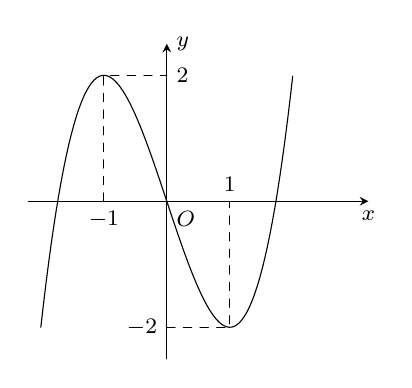
\begin{tikzpicture}[>=stealth,line cap=round,line join=round,font=\footnotesize,scale=.8]
	\draw[->] (-2.2,0)--(3.2,0) node[below] {$x$};
	\draw[->] (0,-2.5)--(0,2.5) node[right] {$y$};
	\node[below right](0,0){$O$};
	\draw[samples=100,domain=-2:2] plot(\x,{(\x)^3-3*(\x)});
	\draw [dashed] (0,-2) node[left]{$-2$} -- (1,-2) -- (1,0) node [above]{$1$};
	\draw [dashed] (-1,0) node[below]{$-1$} -- (-1,2) -- (0,2) node [right]{$2$};
\end{tikzpicture}
}
\loigiai{
Đồ thị đi qua gốc toạ độ nên loại $y=-x^3+3x-2$.\\
Hàm số $y=x^3-3x$ có phương trình $y'=0$ có hai nghiệm $x=1$, $x=-1$.
}
\end{ex}

\begin{ex}%[GHK1, Thái Phiên - Quảng Nam, 2021]%[Phan Tấn Phú - Thành Đức Trung, 12-EX-3-2021]%[2H1Y1-1]
Trong các hình dưới đây, hình nào không phải là hình đa diện?
\begin{center}
\begin{tabular}{c c c c}
	\begin{tikzpicture}[>=stealth,line cap=round,line join=round,font=\footnotesize,scale=.8]
		\coordinate (A) at (0,0);
		\coordinate (B) at (-1,-2);
		\coordinate (C) at (3,-2);
		\coordinate (D) at ($(A)+(C)-(B)$);
		\coordinate (S) at ($(A)+(0,3)$);
		\draw (S) --(B)--(C)--(S)--(D)--(C);
		\draw [dashed] (B)--(A)--(D) (S)--(A);	
	\begin{scope}[on background layer]\path[white]node{MDD-108};\end{scope}
\end{tikzpicture}
	&
	\begin{tikzpicture}[>=stealth,line cap=round,line join=round,font=\footnotesize,scale=.8]
		\coordinate (A) at (0,0);
		\coordinate (B) at (-1,-2);
		\coordinate (C) at (3,-2);
		\coordinate (D) at ($(A)+(C)-(B)$);
		\coordinate (S) at ($(A)+(0,3)$);
		\coordinate (E) at ($(B)+(S)-(A)$);
		\coordinate (F) at ($(C)+(S)-(A)$);
		\coordinate (G) at ($(D)+(S)-(A)$);
		\coordinate (I) at ($(E)+(0.2,1.2)$);
		\coordinate (K) at ($(S)+(0.2,1)$);
		\draw (E)--(I)--(K)--(G) (I)--(F);
		\draw (E)--(B)--(C)--(F)--(E) (C)--(D)--(G)--(F);
		\draw [dashed] (B)--(A)--(D) (S)--(A) (E)--(S)--(G) (S)--(K);
		
	\begin{scope}[on background layer]\path[white]node{MDD-108};\end{scope}
\end{tikzpicture}
	&
	\begin{tikzpicture}[>=stealth,line cap=round,line join=round,font=\footnotesize,scale=.8]
		\coordinate (A) at (0.5,0);
		\coordinate (B) at (-1,-2);
		\coordinate (C) at (3,-2);
		\coordinate (D) at (2,-3);
		\coordinate (S) at ($(A)+(0,3)$);
		\draw (S) --(B)--(C)--(S) (B)--(D)--(C);
		\draw [dashed] (S)--(A)--(B) (A)--(C);
	\begin{scope}[on background layer]\path[white]node{MDD-108};\end{scope}
\end{tikzpicture}
	&
	\begin{tikzpicture}[>=stealth,line cap=round,line join=round,font=\footnotesize,scale=.8]
		\coordinate (A) at (0,0);
		\coordinate (B) at (-1,-2);
		\coordinate (C) at (3,-2);
		\coordinate (D) at ($(A)+(C)-(B)$);
		\coordinate (S) at ($(A)+(0,3)$);
		\coordinate (E) at ($(B)+(S)-(A)$);
		\coordinate (F) at ($(C)+(S)-(A)$);
		\coordinate (G) at ($(D)+(S)-(A)$);
		\draw (S)--(E)--(F)--(G)--(S);
		\draw (E)--(B)--(C)--(F) (C)--(D)--(G);
		\draw [dashed] (B)--(A)--(D) (S)--(A);
	\begin{scope}[on background layer]\path[white]node{MDD-108};\end{scope}
\end{tikzpicture}
	\\
	Hình 1 & Hình 2 & Hình 3 & Hình 4
\end{tabular}
\end{center}
\choice
{Hình 1}
{\True Hình 3}
{Hình 2}
{Hình 4}
\loigiai{
Hình 3 không thoả mãn điều kiện: \lq\lq Mỗi cạnh thuộc một mặt là cạnh chung của đúng hai mặt\rq\rq.
}
\end{ex}

\begin{ex}%[GHK1, Thái Phiên - Quảng Nam, 2021]%[Phan Tấn Phú - Thành Đức Trung, 12-EX-3-2021]%[2H1Y3-3]
Cho tứ diện $ABCD$. Gọi $B'$, $C'$ lần lượt là trung điểm của $AB$, $AC$. Khi đó tỉ số thể tích của khối tứ diện $AB'C'D$ và khối $ABCD$ bằng
\choice
{$\dfrac{1}{6}$}
{\True $\dfrac{1}{4}$}
{$\dfrac{1}{2}$}
{$\dfrac{1}{8}$}
\loigiai{
\immini{
Áp dụng công thức tỉ số thể tích
\[\dfrac{V_{AB'C'D}}{V_{ABCD}}=\dfrac{AB'}{AB}\cdot \dfrac{AC'}{AC}=\dfrac{1}{2}\cdot \dfrac{1}{2}=\dfrac{1}{4}.\]
}{
	\begin{tikzpicture}[>=stealth,line cap=round,line join=round,font=\footnotesize,scale=.8]
	\coordinate (A) at (1,3);
	\coordinate (B) at (0,0);
	\coordinate (C) at (2,-1.5);
	\coordinate (D) at (5,0);
	\coordinate (M) at ($(A)!.5!(B)$);
	\coordinate (N) at ($(A)!.5!(C)$);
	\draw (A)node[above]{$A$}--(B)node[left]{$B$}--(C)node[below]{$C$}--(A)--(D)--(C);
	\draw [dashed] (B)--(D)node[right]{$D$} (M)--(D);	
	\draw (M)node[left]{$B'$}--(N)node[below left]{$C'$}--(D);
\end{tikzpicture}
}
}
\end{ex}

\begin{ex}%[GHK1, Thái Phiên - Quảng Nam, 2021]%[Phan Tấn Phú - Thành Đức Trung, 12-EX-3-2021]%[2D1Y1-2]
Cho hàm số $y=f(x)$ có bảng biến thiên như sau
\begin{center}
	\begin{tikzpicture}[>=stealth,scale=1]
		\tkzTabInit[lgt=1,espcl=2.2]
		{$x$/0.6,$y'$/0.6,$y$/2}{$-\infty$,$-1$,$1$,$+\infty$}
		\tkzTabLine{,+,0,-,0,+,}
		\tkzTabVar{-/$-\infty$,+/$3$,-/$-2$,+/$+\infty$}
	\begin{scope}[on background layer]\path[white]node{MDD-108};\end{scope}
\end{tikzpicture}
\end{center}
Hàm số đồng biến trên khoảng nào dưới đây?
\choice
{$(-1;+\infty)$}
{$(-1;1)$}
{\True $(1;+\infty)$}
{$(-\infty;1)$}
\loigiai{
Hàm số đồng biến trên $(1;+\infty)$.
}
\end{ex}

\begin{ex}%[GHK1, Thái Phiên - Quảng Nam, 2021]%[Phan Tấn Phú - Thành Đức Trung, 12-EX-3-2021]%[2H1Y3-2]
Tính thể tích của khối lập phương có cạnh bằng $a$.
\choice
{$V=\dfrac{a^3}{3}$}
{$V=\dfrac{a^3}{6}$}
{$V=\dfrac{2a^3}{3}$}
{\True $V=a^3$}
\loigiai{
Thể tích khối lập phương cạnh $a$ là $a^3$.
}
\end{ex}

\begin{ex}%[GHK1, Thái Phiên - Quảng Nam, 2021]%[Phan Tấn Phú - Thành Đức Trung, 12-EX-3-2021]%[2D1Y5-3]
\immini{
Cho hàm số $y=f(x)$ có đồ thị như hình vẽ bên. Tìm $m$ để phương trình \(f(x)=m\) có bốn nghiệm phân biệt.
\choice
{\True $-4<m<-3$}
{$m>-4$}
{$-4 \ge m <-3$}
{$-4<m \le -3$}
}{
\begin{tikzpicture}[>=stealth,line cap=round,line join=round,font=\footnotesize,scale=.8]
	\draw[->] (-2.5,0)--(2.5,0) node[below] {$x$};
	\draw[->] (0,-5)--(0,2) node[right] {$y$};
	\node[below right](0,0){$O$};
	\draw[samples=100,domain=-1.8:1.8] plot(\x,{(\x)^4-2*(\x)^2-3});
	\draw [dashed] (-1,0) node[above]{$-1$} -- (-1,-4) -- (0,-4) node [below left]{$-4$}--(1,-4)--(1,0) node [above]{$1$};
	\draw (0,-3) node [right]{$-3$};
\end{tikzpicture}
}
\loigiai{
Phương trình $f(x)=m$ là phương trình hoành độ giao điểm của đồ thị hàm số $y=f(x)$ và đường thẳng $y=m$. Từ hình vẽ ta có phương trình có 4 nghiệm phân biệt khi $-4<m<-3$.
}
\end{ex}

\Closesolutionfile{ans}

\begin{indapan}{10}
	{ans/ans-2-GHK1-34-ThaiPhien-QuangNam-21}
\end{indapan}